\documentclass{article}
\usepackage{anyfontsize}
\usepackage{graphicx}
\usepackage{hyperref}
\usepackage{parskip}
\usepackage[section]{placeins}

\fontsize{10pt}{12pt}\selectfont % Set the font size
\begin{document}

% FRONT PAGE
\begin{titlepage}
    \begin{center}
        
        Politecnico di Milano\\
      
        Computer Science and Engineering\\
        
        Software Engineering II\\

        \vfill
        
        {\Large \textbf{RASD - CodeKataBlade}}\\
        
        \vfill

        José Alejandro Sarmiento

        \today

        v1.0
        
    \end{center}
\end{titlepage}
\newpage


% TABLE OF CONTENTS
\tableofcontents


\section{INTRODUCTION}
\subsection{Purpose}

The primary purpose of the CodeKataBattle (CKB) platform is to provide an environment 
for students to enhance their software development skills through collaborative 
learning and friendly competition and for educators to set up these scenarios. The platform facilitates 
this by allowing educators to setup tournaments where code kata battles are organized. Here students 
form teams and showcase their coding abilities in a test-driven development (TDD) framework.

\textbf{A) Skill Enhancement through Practice:}

CKB serves as a virtual arena where students can test and improve their programming abilities by actively 
participating in code kata battles.

\textbf{B) Educator-Guided Learning:}

The platform must allow for educators to create tournaments, compose battles and perform manual evaluations
on top of automated ones. This ensures that the learning experience aligns with the curriculum and instructional goals.

\textbf{C) Automated Evaluation:}

CKB should have an automated evaluation system that provides feedback to students based on
 objective criteria. Specifically, the criteria the evaluation is based upon is the number of passed test cases 
 set up by the battle organizer and the timeliness. 

 \textbf{D) Competition and Recognition:}

The platform should possess a leaderboard functionality that allows participants to 
gauge their performance and see how their skills compare to other participants.

In summary, CodeKataBattle aims to create a learning platform, combining 
hands-on coding practice, collaborative teamwork and automated feedback, all under the 
guidance of educators. 

Knowing this, the S2B will have a certain set of goals to achieve:
\begin{itemize}
    \item \textbf{G1:} Every educator should be able to create a tournament.
    \item \textbf{G2:} When crearing a tournament, the educator doing so should be able to set a registration deadline.
    \item \textbf{G3:} Every educator that owns a tournament should be able to invite other educators to it.
    \item \textbf{G4:} Every educator that belongs to a tournament should be able to create battles.
    \item \textbf{G5:} When creating a battle, the educator doing so should be able to set the programming language, a decription of the problem, the test cases which will evaluate the students code, the build automation scripts, the registration deadline, the final submission deadline, the minimum and maximum number of participants per group.
    \item \textbf{G6:} Every student should be able to see the list of tournaments and register to them before the registration deadline.
    \item \textbf{G7:} Every student should be able to see the description of the battles of a tournament they belong to and register to them before the registration deadline by themselves or with other students by inviting them to join or by accepting another student's invitation.
    \item \textbf{G8:} Every time a student makes a submission to a battle, the platform should evaluate it and update the leaderboard of the battle accordingly.
    \item \textbf{G9:} The evaluation carried on by the platform should be performed with the build automation scripts set by the educator and should be based on the test cases set by the educator and the timeliness of the submission.
    \item \textbf{G10:} Every student and educator should be able to see the leaderboard of a battle they belong to.
    \item \textbf{G11:} Once the battle ends, the educator that created it should be able to manually evaluate the code of the students if they so desire to and set a grade for each student.
    \item \textbf{G12:} Once the educator consolidates the results of a battle, the students that participated in it should be notified, the final results of the battle should be displayed to everyone. The leaderboard of the tournament the battle belongs to should be updated by adding for each student the battle score to the sum of all the other battles they have participated on.
    \item \textbf{G13:} Every student and educator should be able to see the leaderboard of every tournament.
    \item \textbf{G14:} An instructor that owns a tournament should be able to close it.
    \item \textbf{G15:} Once the owner of a tournament closes it, the platform should notify all the students once the leaderboard of the tournament is available.
    \item \textbf{G16:} When a tournament is created, all students should be notified. 
    \item \textbf{G17:} When a battle is created, all students participating in the tournament the battle belongs to should be notified.
\end{itemize}

\newpage

\subsection{Scope}  

The education sector in software development is an ever-growing field given the nature of the topic 
being teached. 

The CodeKataBattle (CKB) platform aims to provide a competitive twist to the learning
by facilitating the creation of competitions in the form of tournaments where students can showcase their abilities.

These are managed by educators who can create the aforementioned tournaments and compose battles where they can decide 
the programming language, the description of the problem and the test cases which will evaluate the students code among other things.

This way, through the use of GitHub, the platform can automatically evaluate the code of a team.

In the environment of the CodeKataBattle system the following actors are identified:

\textbf{Students:} These are the primary users of the CKB system. They participate in battles and tournaments to improve their software development skills. They can form teams, work on code katas, and submit their solutions.

\textbf{Educators:}: They are responsible for creating and managing battles and tournaments. They set various parameters for battles, evaluate the solutions submitted by students, and provide feedback.

\textbf{GitHub:} The CKB system integrates with GitHub for managing code kata projects and tracking students' commits. GitHub is a widely used platform for version control and collaboration in software development.

Having all of this in mind, the following are the World and Shared phenomena that the system will have to deal with:

\textbf{World Phenomena:}

\begin{itemize}
    \item \textbf{W1:} A group of students organizes themselves to participate in a battle together.
    \item \textbf{W2:} A group of students registered to a battle fork the repository of the battle.
    \item \textbf{W3:} Students set up an automated workflow through GitHub Actions that will notify the system every time a commit is pushed to the main branch of the forked repository of a battle.
    \item \textbf{W4:} A student pushes a commit to the main branche of a forked repository of a battle.
    \item \textbf{W5:} An educator possesses a specific evaluation criteria through which they perform their manual evaluations.
\end{itemize}

\textbf{Shared Phenomena:}

Controlled by the world and observed by the system.

\begin{itemize}
    \item \textbf{SP1:} An educator creates a tournament with a set of attributes.
    \item \textbf{SP2:} An educator creates a battle with a set of attributes inside a tournament.
    \item \textbf{SP3:} An educator invites other educators to a tournament.
    \item \textbf{SP4:} A student registers to a tournament.
    \item \textbf{SP5:} A student or a team of students registers to a battle.
    \item \textbf{SP6:} GitHub notfies the system that a student has pushed a commit to the main branch of a forked repository of a battle. 
    \item \textbf{SP7:} An educator performs manual evaluations on the submissions of a battle they own.
    \item \textbf{SP8:} An educator consolidates the results of a battle.
    \item \textbf{SP9:} An educator closes a tournament.
\end{itemize}

Controlled by the system and observed by the world.

\begin{itemize}
    \item \textbf{SP10:} The system notifies all the students that a tournament has been created.
    \item \textbf{SP11:} The system notifies all the students participating in a tournament that a battle has been created.
    \item \textbf{SP12:} The system displays the leaderboard of tournament while it is active and after it has ended.
    \item \textbf{SP13:} The system displays the leaderboard of a battle while it is active and after it has ended.
    \item \textbf{SP14:} The system updates a battle's leaderboard every time a new evaluation is performed.
    \item \textbf{SP15:} The system notifies all the students participating in a battle that the final results have been consolidated.
    \item \textbf{SP16:} The system updates the leaderboard of a tournament every time a battle ends.
    \item \textbf{SP17:} The system notifies all the students participating in a tournament that it has ended.
\end{itemize}

\newpage

\subsection{Definitions, Acronyms, Abbreviations}

\subsubsection{Definitions}
 
\begin{itemize}
    \item \textbf{Tournament:} A tournament is a space where educators can create battles and students can register to them. It has a registration deadline and a leaderboard that is updated every time a battle ends.
    \item \textbf{Battle:} A battle is a space where students can register to and submit their solutions to a problem. It has a registration deadline, a final submission deadline, a leaderboard that is updated every time a new evaluation is performed and a set of test cases that will be used to evaluate the submissions.
    \item \textbf{GitHub:} GitHub is a code hosting platform for version control and collaboration. It lets you and others work together on projects from anywhere.
    \item \textbf{GitHub Actions:} GitHub Actions is a CI/CD tool that allows you to automate your software development workflows in the same place you store code and collaborate on pull requests and issues.
    \item \textbf{Educator:} An educator, in the context of the system, is a user of the platform that can create tournaments and battles, invite other educators to tournaments, perform manual evaluations on the submissions of a battle they own and consolidate the results of a battle.
    \item \textbf{Student:} A student, in the context of the system, is a user of the platform that can register to tournaments and battles, create teams and submit their solutions to a battle.
    \item \textbf{Build Automation Scripts:} Build automation scripts are scripts that are run automatically by the system every time a commit is pushed to the main branch of the forked repository of a battle. They are used to evaluate the submissions of the students.
    \item \textbf{Test Case:} A test case is a set of conditions under which a tester will determine whether an application, software system or one of its features is working as it was originally established for it to do.
    \item \textbf{Timeliness:} Timeliness is the quality of doing something or producing something at the right time. In the context of the system, it refers to the time in which a student submits their solution to a battle with respect to the start of the battle and the final submission deadline.
\end{itemize}

\subsubsection{Acronyms}

\begin{itemize}
    \item \textbf{CKB:} CodeKataBattle
    \item \textbf{S2B:} System to Be
    \item \textbf{TDD:} Test-Driven Development
    \item \textbf{CI/CD:} Continuous Integration/Continuous Delivery
    \item \textbf{UI:} User Interface
    \item \textbf{API:} Application Programming Interface
    \item \textbf{UML:} Unified Modeling Language
\end{itemize}

\subsubsection{Abbreviations}

\begin{itemize}
    \item \textbf{Gn:} Goal number n
    \item \textbf{Wn:} World Phenomena number n
    \item \textbf{SPn:} Shared Phenomena number n
    \item \textbf{Dn:} Domain Assumption number n
    \item \textbf{Rn:} Requirement number 
    \item \textbf{UCn:} Use Case number n
\end{itemize}


\subsection{Revision history}
\subsection{Reference Documents}

The specification of the RASD and DD assignment of the Software
Engineering II course, held by professor Matteo Rossi, Elisabetta Di Nitto and
Matteo Camilli at the Politecnico di Milano, A.Y 2023/2024;

\subsection{Document Structure}

\begin{itemize}
    \item \textbf{1. Introduction:} This section provides an overview of the entire document. It identifies the product’s goals and the scope of the system along with the definitions, acronyms, abbreviations and the revision history.
    \item \textbf{2. Overall Description:} This section provides a general description of the product and its functionality. It also describes the user characteristics, assumptions, dependencies and constraints.
    \item \textbf{3. Specific Requirements:} This section contains all the software requirements to a level of detail sufficient to enable designers to design a system to satisfy those requirements, and testers to test that the system satisfies those requirements.
    \item \textbf{4. Formal Analysis Using Alloy:} This section contains a formal analysis of the system using the Alloy language.
    \item \textbf{5. Effort Spent:} This section contains the number of hours each group member has worked on the document.
    \item \textbf{6. References:} This section contains all the reference documents used to create this document.
\end{itemize}

\section{OVERALL DESCRIPTION}
\subsection{Product perspective}
\subsubsection{Scenarios}

\begin{itemize}
    \item \textbf{1. Educator creates a tournament:} 
    
    An educator called Adam wants to create a tournament for his students. He goes to the CKB platform and creates a tournament with a registration deadline of 2 weeks from now. The platform notifies all the students that a tournament has been created. He then invites his colleagues to the tournament so when the tournament starts they can create battles.

    \textbf{Goals:} G1, G2, G3, G16.
    \textbf{Phenomena:} SP1, SP3, SP10.

    \item \textbf{2. Student registers to a tournament:}
    
    A student called Bob receives a notification that a tournament has been created by educator Adam. He goes to the CKB platform and registers to the tournament before the registration deadline.

    \textbf{Goals:} G6, G16.
    \textbf{Phenomena:} SP4, SP10.

    \item \textbf{3. Educator creates a battle:}
    
    Educator Charlie wants to create a battle for the tournament he was invited to by educator Adam. He goes to the CKB platform and creates a battle with a registration deadline of 1 week from now, a final submission deadline of 2 weeks from now, a minimum of 1 participant per group and a maximum of 3 participants per group. He also sets the programming language to Java, the description of the problem and uploads the build automation scripts and test cases which will evaluate the students code. The platform notifies all the students participating in the tournament that a battle has been created.

    \textbf{Goals:} G4, G5, G17.
    \textbf{Phenomena:} SP2, SP11.

    \item \textbf{4. Students registers to a battle:}
    
    Bob receives a notification that a battle has been created by educator Charlie. He goes to the CKB platform and reads the description of the battle. He then contacts his friends Danielle and Eve, who are also inside educator Adam's tournament, and they decide to form a team and register to the battle together. Charlie invites Danielle and Eve to the battle and they accept. 

    \textbf{Goals:} G7, G17.
    \textbf{Phenomena:} W1, SP5, SP11.

    \item \textbf{5. Student submits a solution to a battle:}
    
    After the registrarion deadline ends, the system sends the link to the newly created GitHub repository to the students that registered to the battle. Bob, Danielle and Eve fork the repository and set up an automated workflow through GitHub Actions that will notify the system every time a commit is pushed to the main branch of the forked repository of the battle. After that, they start working on the problem and push a commit to the main branch of the forked repository of the battle. The system receives the notification thanks to the automated workflow and runs the build automation script to evaluate the submission taking into account the test cases educator Charlie submitted and the timeliness of the submission. The system then updates the leaderboard of the battle accordingly. The team notices that they have not passed all the test cases and decide to keep working on the problem. After a few days of several teams submitting their solutions, educator Charlie checks the leaderboard to see how the students are doing.

    \textbf{Goals:} G8, G9, G10.
    \textbf{Phenomena:} W2, W3, W4, SP6, SP13, SP14.

    \item \textbf{6. Educator performs manual evaluations on the submissions of a battle after it has ended:}
    
    After the final submission deadline of educator Charlie's battle ends, he decides to manually evaluate the submissions of the students. He sets a grade for each team based on his own evaluation criteria. After that, he consolidates the results of the battle. The system updates the leaderboards taking into account the evaluation it performed and the evaluations from educator Charlie. It then also updates the tournament leadeaboard accordingly. The system then notifies all the students participating in the battle that the final results have been consolidated. Bob, Danielle and Eve check the leaderboard and see their score. They then check the leaderboard of the tournament and see that their score has been added to the sum of all the other battles they have participated on.

    \textbf{Goals:} G11, G12, G13.
    \textbf{Phenomena:} W5, SP7, SP8, SP12, SP13, SP15, SP16.

    \item \textbf{7. Educator closes a tournament:}
    
    After all the battles of the tournament have ended, educator Adam decides to close the tournament. The system notifies all the students participating in the tournament that it has ended. Bob, Danielle and Eve check the leaderboard of the tournament and see their final score.

    \textbf{Goals:} G14, G15.
    \textbf{Phenomena:} SP9, SP17.


\end{itemize}
\newpage
\subsubsection{Domain Class Diagram}

In Figure 1 we can see the Domain Class Diagram of the system.

In it we can see the following classes:

\begin{itemize}
    \item \textbf{Student:} This class represents a student of the platform. It has an id, a name, a github account and it associates to a set of TournamentRegistrations and StudentTeams.
    \item \textbf{TournamentRegistration:} This class represents a registration of a student to a tournament. It saves the score the associated student has on the associated tournament. Serves as a Many to Many relationship between Student and Tournament.
    \item \textbf{StudentTeam:} This class represents a team of students. There can be 1 or more students in one StudentTeam. It has an id and saves the score of the team on the battle the team belongs to.
    \item \textbf{Tournament:} This class represents a tournament. It has an id and a registration deadline. It is associated to a set of Battles and TournamentRegistrations. It also has an owner which is an Educator and a set of invited educators.
    \item \textbf{Battle:} This class represents a battle. It has an id, a registration deadline, a final submission deadline, and a minimum and maximum number of participants per group. It belongs to a tournament and it contains a set of StudentTeams, a CodeKata and a GitHubRepo.
    \item \textbf{CodeKata:} This class represents a code kata. It has a programming language, a description, a set of test cases and a set of build automation scripts. These will be uploaded to the GitHubRepo of the battle. 
    \item \textbf{GitHubRepo:} This class represents a GitHub repository. It has an id and it belongs to a battle. 
    \item \textbf{GitHubIntegration:} This class represents the integration of the system with GitHub. It could act as a facade for the GitHub API.
    \item \textbf{Educator:} This class represents an educator of the platform. It has an id, a name, and it associates to a set of Tournaments and Battles. It can associato to tournaments as an owner or as an invited educator. 
\end{itemize}
\newpage
\begin{figure}[h]
    \centering
    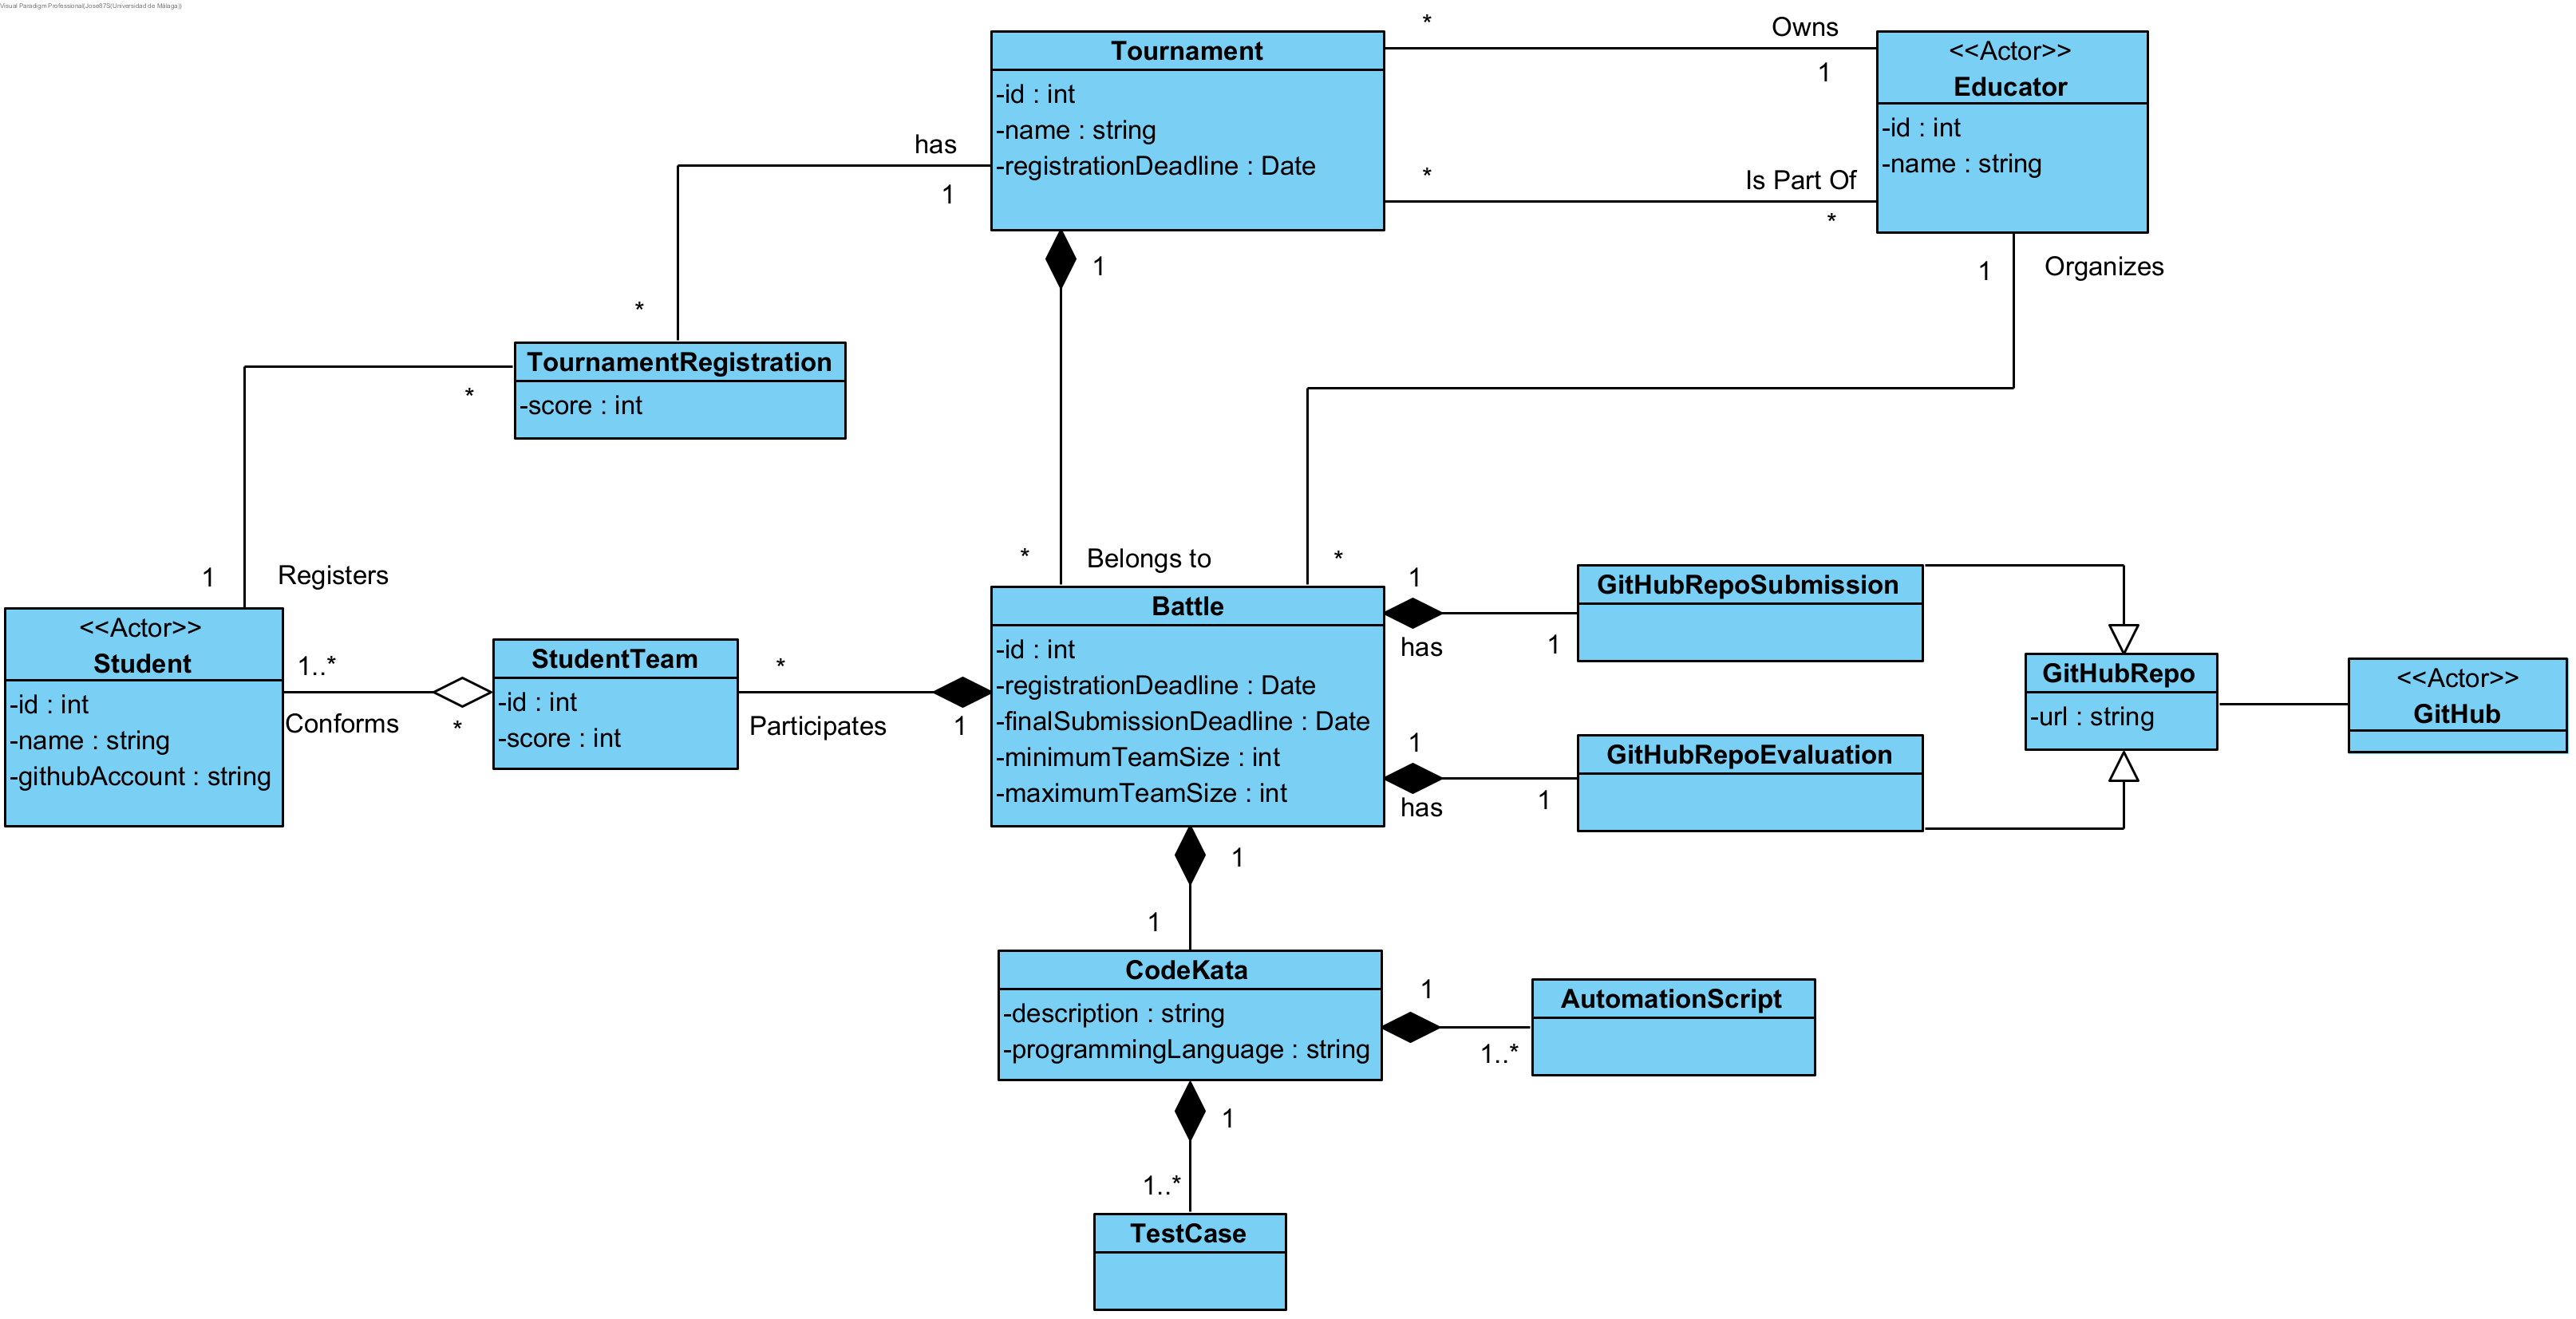
\includegraphics[width=1\textwidth]{images/DomainClassDiagram.png}
    \caption{Domain Class Diagram}
    \label{fig:DomainClassDiagram}
\end{figure}

\subsubsection{State Diagrams}

Here it is possible to see the state diagrams for the classes of the system where this is more relevant.
\begin{itemize}
    \item \textbf{Battle:}
\end{itemize}

\begin{figure}[!h]
    \centering
    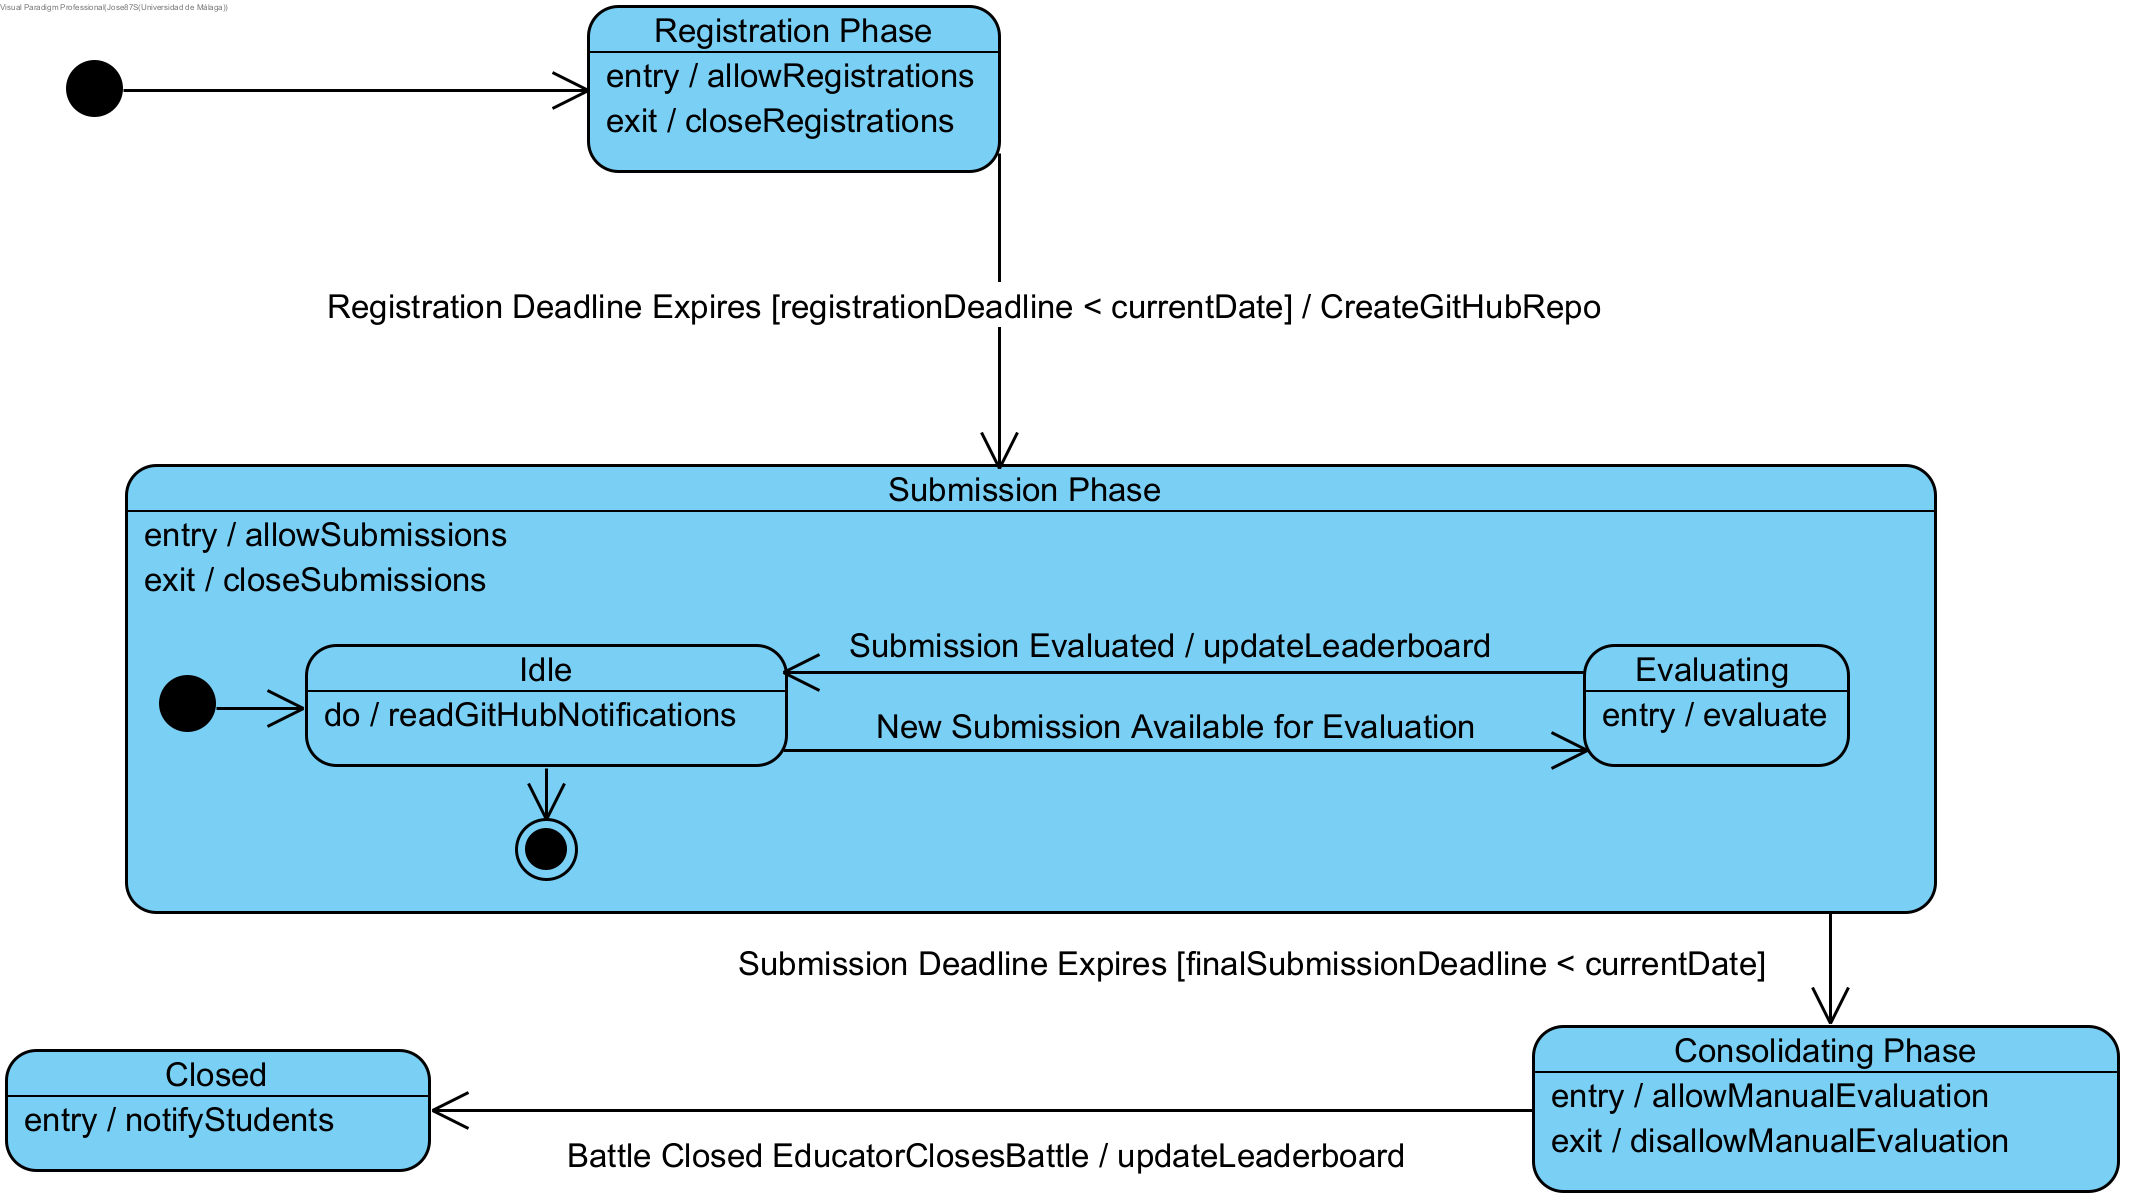
\includegraphics[width=1\textwidth]{images/BattleStateDiagram.png}
    \caption{Battle State Diagram}
    \label{fig:BattleStateDiagram}
\end{figure}

A battle is firstly on it's \textbf{Registration Phase} where StudentTeams can register to 
it. Once the registration deadline is reached, the battle moves to the 
\textbf{Submission Phase} and it creates the \textbf{GitHubRepo}. Here the \textbf{StudentTeam}s  
can submit their solutions to the battle 
through GitHub. In this state there are two substates: \textbf{Idle} and \textbf{Evaluating}. 
In the \textbf{Idle} state, the system is waiting for a notification from GitHub that a commit 
has been pushed to the main branch of one of the forked repositories of the battle. Once the system 
receives the notification, it moves to the \textbf{Evaluating} state where it runs the build 
automation scripts to evaluate the submission. Once the evaluation is done, the system updates 
the leaderboard of the battle and moves back to the \textbf{Idle} state. Once the final submission 
deadline is reached, the battle moves to the \textbf{Consolidation Phase} where the \textbf{Educator} that 
created the battle can perform manual evaluations on the submissions of the \textbf{Student}s. 
Once the \textbf{Educator} consolidates the results of the battle, the battle moves to the \textbf{Closed} 
state updating the leaderboard of the battle with the \textbf{Educator}'s evaluations. Here the system 
notifies the \textbf{Student}s that the final results have been published.

\begin{itemize}
    \item \textbf{Tournament:}
\end{itemize}

\begin{figure}[!h]
    \centering
    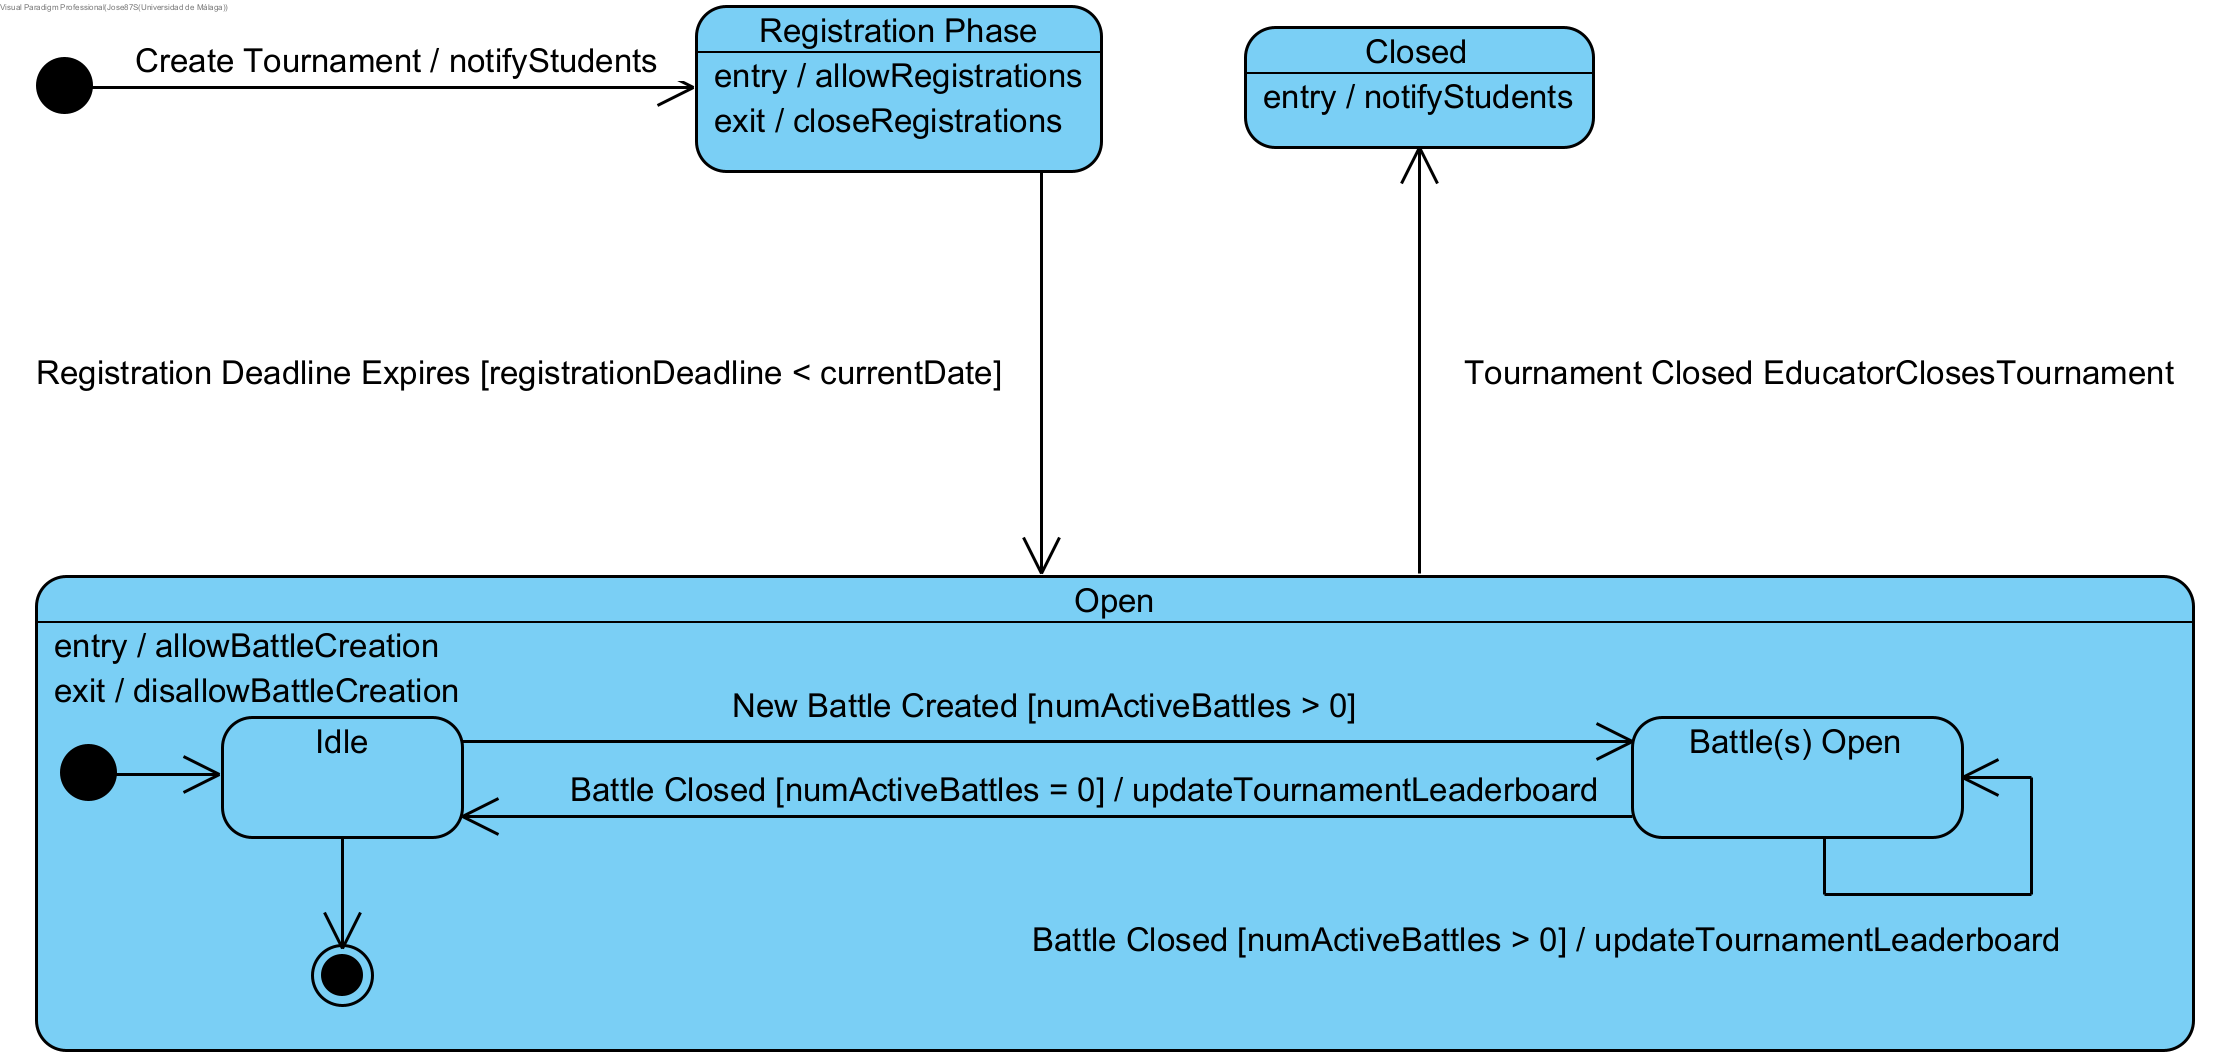
\includegraphics[width=1\textwidth]{images/TournamentStateDiagram.png}
    \caption{Tournament State Diagram}
    \label{fig:TournamentStateDiagram}
\end{figure}

When a \textbf{Tournament} is created, all students are notified. A \textbf{Tournament}, similar a \textbf{Battle}, has a \textbf{Registration Phase} where \textbf{Student}s can register to it.
Once the registration deadline is reached, the \textbf{Tournament} moves to the \textbf{Open} state. Here all the \textbf{Educator}s
that are part of the \textbf{Tournament} can create \textbf{Battle}s. The \textbf{Open} state has two substates: \textbf{Idle} 
and \textbf{Battle(s) Open}. In the \textbf{Idle} state, there are no active \textbf{Battle}s in the \textbf{Tournament}. Once an
\textbf{Educator} creates a battle, the \textbf{Tournament} moves to the \textbf{Battle(s) Open} state. Each time a battle ends,
the \textbf{Tournament} leaderboard is updated. The \textbf{Tournament} moves back to the \textbf{Idle} state once there are no active \textbf{Battle}s.
The \textbf{Tournament} can move to the closed state once the owner of the \textbf{Tournament} decides to close it and there are no active \textbf{Battle}s. 
Here, \textbf{Student}s are notified that the final results are available.

\subsection{Product functions}

\begin{itemize}
    \item \textbf{Sign up and Login:}
    
    This is a basic functionality of the system. It allows for students and educators to sign up and login to the system.
    When signing up, the user must provide a name, an email, a password and a GitHub account. The system will then send a confirmation email to the user.
    Once the user confirms their email, they can login to the system.

    \item \textbf{Create Tournament:}
    
    This functionality allows for educators to create tournaments. When creating a tournament, the educator
    must provide a registration deadline and can invite other educators to the tournament. Once the tournament
    is created, the system will notify all the students that a tournament has been created. 

    \item \textbf{Register to Tournament:}
    
    This functionality allows for students to register to tournaments. When registering to a tournament which is on 
    its registration phase. Students are able to join all the tournaments which are on this phase.

    \item \textbf{Create Battle:}
    
    This functionality allows for educators to create battles. When creating a battle, the educator
    must provide a registration deadline, a final submission deadline, a minimum and maximum number of participants per group, 
    a programming language, a description of the problem, a set of test cases and a set of build automation scripts. 
    Once the battle is created, the system will notify all the students participating in the tournament that 
    a battle has been created. The system will use the files provided by the educator to create a GitHub repository for the battle.
    
    \item \textbf{Register to Battle:}
    
    This functionality allows for students to register to battles. When registering to a battle, which is on
    its registration phase, students can invite other students or accept invitations from other students to join the battle,
    always taking into account the minimum and maximum number of participants per group set by the educator.

    \item \textbf{Evaluate submissions:}
    
    This functionality allows for the system to evaluate the submissions of the students. Each time the system receives
    a notification from GitHub that a commit has been pushed to the main branch of one of the forked repositories of the battle,
    the system will pull the latest sources, run the tests and update the leaderboard of the battle accordingly.

    \item \textbf{Consolidate results:}
    
    Once the final submission deadline of a battle ends, the educator that created the battle can consolidate the 
    results of the battle. This means that the educator can manually evaluate the submissions of the students and 
    set a grade for each team, which will be combined with the evaluation performed by the system. Once the educator
    finishes consolidating the results, the system will update the leaderboard of the battle and notify all the students.

    \item \textbf{Close Tournament:}
    
    Once all the battles of a tournament have ended, the owner of the tournament can close it. This means that the
    system will update the leaderboard of the tournament and notify all the students that the tournament has ended.
\end{itemize}

\subsection{User characteristics}

\begin{itemize}
    \item \textbf{Students:} They participate in battles and tournaments to improve their software development skills. They can form teams, work on the battles, and submit their solutions through GitHub.
    \item \textbf{Educators:}: They are responsible for creating and managing battles and tournaments. They set various parameters for battles, evaluate the solutions submitted by students, and provide feedback.
\end{itemize}

\newpage
\subsection{Assumptions, dependencies and constraints}

\subsubsection{Domain Assumptions}

\begin{itemize}
    \item \textbf{D1:} All users have a valid email address and can access their email to confirm their registration.
    \item \textbf{D2:} GitHub integration is reliable, and the system can communicate with GitHub to create repositories, pull code, and receive notifications.
    \item \textbf{D3:} Students and educators have a basic understanding of version control systems, especially GitHub.
    \item \textbf{D4:} Educators have the necessary expertise to create meaningful and effective code kata battles, including defining appropriate test cases.
    \item \textbf{D5:} Students have the required technical skills to participate in code kata battles, including forking repositories, setting up GitHub Actions, and writing code.
    \item \textbf{D6:} The system has access to resources (computational resources, storage, etc.) to perform automated evaluations of code submissions.
    \item \textbf{D7:} Users have a GitHub account.
    \item \textbf{D8:} The educator's uploaded description of the problem, programming language test cases and build automation scripts are all related to each other.
    \item \textbf{D9:} Educators have a set of evaluation criteria through which they perform their manual evaluations.
\end{itemize}

\subsubsection{Dependencies}

\begin{itemize}
    \item The system relies on GitHub for version control, code repository management, and continuous integration through GitHub Actions.
    \item Email services are required for user registration confirmation and communication.
\end{itemize}

\subsubsection{Constraints}

\begin{itemize}
\item The system's functionality heavily depends on the reliability and availability of external services such as GitHub and email services.
\item The system's performance is constrained by the response time of GitHub services for repository creation and code evaluation.
\item Users must have internet access to interact with the CKB platform and GitHub services.
\end{itemize}

\section{SPECIFIC REQUIREMENTS}
\iffalse
    \item \textbf{G1:} Every educator should be able to create a tournament.
    \item \textbf{G2:} When crearing a tournament, the educator doing so should be able to set a registration deadline.
    \item \textbf{G3:} Every educator that owns a tournament should be able to invite other educators to it.
    \item \textbf{G4:} Every educator that belongs to a tournament should be able to create battles.
    \item \textbf{G5:} When creating a battle, the educator doing so should be able to choose the programming language.
    \item \textbf{G6:} When creating a battle, the educator doing so should be able to set a decription of the problem.
    \item \textbf{G7:} When creating a battle, the educator doing so should be able to set the test cases which will evaluate the students code.
    \item \textbf{G8:} When creating a battle, the educator doing so should be able to set the registration deadline.
    \item \textbf{G9:} When creating a battle, the educator doing so should be able to set the final submission deadline.
    \item \textbf{G10:} When creating a battle, the educator doing so should be able to set the minimum and maximum number of participants per group.
    \item \textbf{G11:} The platform should be able to create a GitHub repository for each battle after the registration deadline.
    \item \textbf{G12:} The platform should send invitations to the GitHub repository of a battle to the students that registered to it.
    \item \textbf{G13:} Every student should be able to see the list of tournaments.
    \item \textbf{G14:} Every student should be able to register to a tournament before the registration deadline.
    \item \textbf{G15:} Every student and educator should be able to see the description of the battles of a tournament they belong to.
    \item \textbf{G16:} Every student should be able to register to a battle of a tournament they are a part of by themselves or with other students before the battle's registration deadline.
    \item \textbf{G17:} The platform should be able to automatically evaluate the code of a student every time a commit is pushed to the main branch of the forked repository of a battle.
    \item \textbf{G18:} The evaluation carried on by the platform should be based on the test cases set by the educator and the timeliness of the submission.
    \item \textbf{G19:} The platform should be able to update the leaderboard of a battle every time an evaluation is performed. 
    \item \textbf{G20:} Every student and educator should be able to see the leaderboard of a battle they belong to.
    \item \textbf{G21:} Once the battle ends, the educator that created it should be able to manually evaluate the code of the students if they so desire to.
    \item \textbf{G22:} Once the educator consolidates the results of a battle, the students that participated in it should be notified.
    \item \textbf{G23:} Once the educator consolidates the results of a battle, the final results of the battle shoud be displayed to everyone.
    \item \textbf{G24:} Once the educator consolidates the results of a battle, the tournament leaderboard should be updated by adding the score that each student got on the battle to their score on the rest of the battles of the tournament that they have participated on.
    \item \textbf{G25:} Every student and educator should be able to see the leaderboard of every tournament.
    \item \textbf{G26:} An instructor that owns a tournament should be able to close it.
    \item \textbf{G26:} Once the owner of a tournament closes it, the platform should notify all the students once the leaderboard of the tournament is available.
\fi
\subsection{External Interface Requirements}
\subsubsection{User Interfaces}
\subsubsection{Hardware Interfaces}
\subsubsection{Software Interfaces}
\subsubsection{Communication Interfaces}
\subsection{Functional Requirements}
\subsection{Performance Requirements}
\subsection{Design Constraints}
\subsubsection{Standards compliance}
\subsubsection{Hardware limitations}
\subsubsection{Any other constraint}
\subsection{Software System Attributes}
\subsubsection{Reliability}
\subsubsection{Availability}
\subsubsection{Security}
\subsubsection{Maintainability}
\subsubsection{Portability}

\section{FORMAL ANALYSIS USING ALLOY}

\section{EFFORT SPENT}

\section{REFERENCES}

\end{document}

